\documentclass[aspectratio=1610]{beamer}

\usepackage{graphicx}
\usepackage[english]{babel}
\usepackage[T1]{fontenc}
\usepackage{csquotes, xcolor, xspace, changepage, setspace, listings}
\usepackage{libertinus}
\usepackage{roboto}
\usepackage{fontawesome5}
\usepackage[scale = 0.75]{plex-mono}
\usepackage{tikz, subcaption}

\usetikzlibrary{fit, shapes.geometric, shapes.symbols, positioning, shapes.misc, calc, arrows.meta, patterns, backgrounds, decorations, decorations.markings, decorations.pathreplacing, shadows, hobby}

\usepackage[backend=bibtex,style=authoryear]{biblatex}
\addbibresource{biblio.bib}

\title{Markerless 3D Human Pose Tracking}
\author{Roland Bernard}
\date{September 2026}

\definecolor{unibzblue}{HTML}{0086ec}
\definecolor{unibzblue2}{HTML}{f0f8ff}

\setbeamercolor{outerbox}{fg=black,bg=unibzblue2}
\setbeamercolor{innerbox}{fg=white,bg=unibzblue}

\setbeamertemplate{title page}{
  \scriptsize 
  \begin{tabular}{ll}
    \vspace*{45mm} \\
    \multicolumn{2}{l}{\raggedright Project Presentation -- Capstone Project 2025/2026} \\
    \\
    \multicolumn{2}{p{\linewidth}}{\raggedright \huge \bf \inserttitle} \\
    \\
    \\
    \begin{tabular}{rl}
    & \insertauthor \\
    & \\
    \tiny Tutor & Oswald Lanz \\
    \tiny Domain Expert & Marco Boschetti (Covision Lab) \\
    & \\
    \tiny Date & \insertdate \\
    \end{tabular}
  \end{tabular}
}

\setbeamertemplate{frametitle}{
  \vspace*{6mm}
  \Large \bf \color{black} \insertframetitle
}

\setbeamertemplate{itemize items}{\scriptsize\raisebox{0.6mm}{\color{unibzblue} $\blacktriangleright$}}

\beamertemplatenavigationsymbolsempty
\setbeamertemplate{footline}{
  \begin{beamercolorbox}[wd=\paperwidth,right]{section in head/foot}
    \usebeamerfont{date in head/foot}\hspace*{2em}
    \insertframenumber{}\hspace*{2mm} 
    \vspace*{2mm}
  \end{beamercolorbox}
}

\newcommand{\litem}{{\scriptsize\raisebox{0.6mm}{\color{unibzblue} $\blacktriangleright$}}}
\newcommand{\sitem}{{\scriptsize\raisebox{0.2mm}{\color{unibzblue} $\rightarrow$}}\enspace}
\newcommand{\icon}[1]{\textcolor{unibzblue}{\faIcon[solid]{#1}}}

\newlength{\offsetpage}
\newenvironment{narrowpage}[1][3mm]{
  \setlength{\offsetpage}{#1}
  \begin{adjustwidth}{\offsetpage}{\offsetpage}
}{
  \end{adjustwidth}
}
\newenvironment{widepage}[1][10mm]{
  \setlength{\offsetpage}{#1}
  \begin{adjustwidth}{-\offsetpage}{-\offsetpage}
}{
  \end{adjustwidth}
}

\newenvironment{items}{
  \begin{narrowpage}
}{
  \end{narrowpage}
}
\newenvironment{oitem}[2][3mm]{
  \vspace*{2mm}
  \begin{beamercolorbox}[rounded=false,colsep=#1]{outerbox}
    \parbox[t]{2mm}{\centering#2}\parbox[t]{2mm}{\ }%
    \begin{minipage}[t]{\linewidth}
}{
    \end{minipage}
  \end{beamercolorbox}
  \vfill
}

\input{tikzfigures/defs.tex}

\begin{document}

\begin{frame}[plain]
  \begin{tikzpicture}[
    remember picture, overlay,
    every path/.style={opacity=0.10},
    yshift=20, xshift=200, scale=1.5, transform shape
  ]
    \node {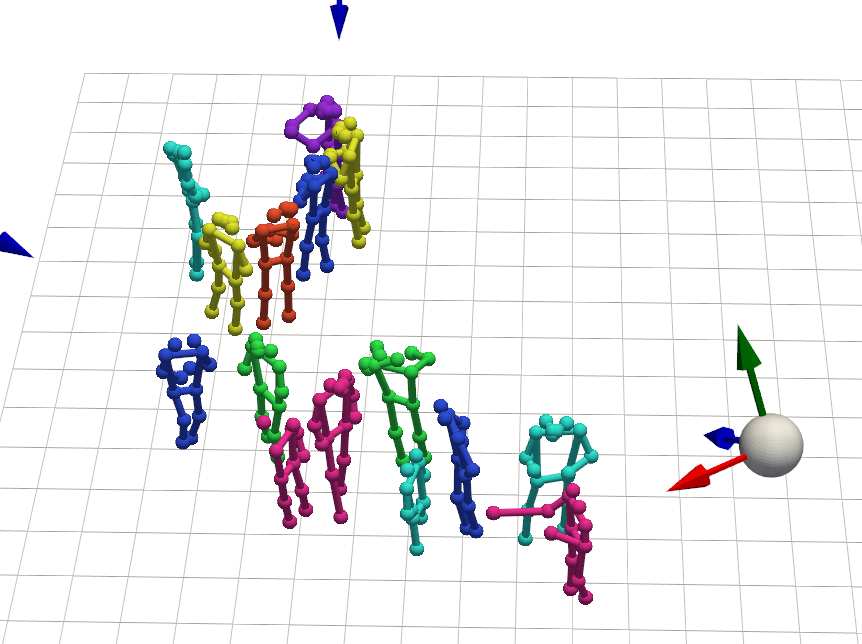
\includegraphics[width=0.9\linewidth]{figures/background.png}};
  \end{tikzpicture}
  \titlepage
\end{frame}

\begin{frame}
\frametitle{Introduction}
  \begin{items}
    \begin{oitem}{\litem}
      Problem: {\footnotesize Track poses of multiple people in videos across multiple views.}
    \end{oitem}
    \begin{oitem}{\litem}
      Possible Applications: \\
      \sitem {\footnotesize Robotics and human-robot interactions.} \\
      \sitem {\footnotesize In healthcare, for tasks such as gait analysis or remote patient monitoring.} \\
      \sitem {\footnotesize For real-time motion capture or natural body-based control interfaces for gaming.}
    \end{oitem}
    \begin{oitem}{\litem}
      Objectives of this project: \\
      \sitem {\footnotesize Develop and evaluate a 3D pose tracking pipeline.}
    \end{oitem}
    \begin{figure}
      \centering
      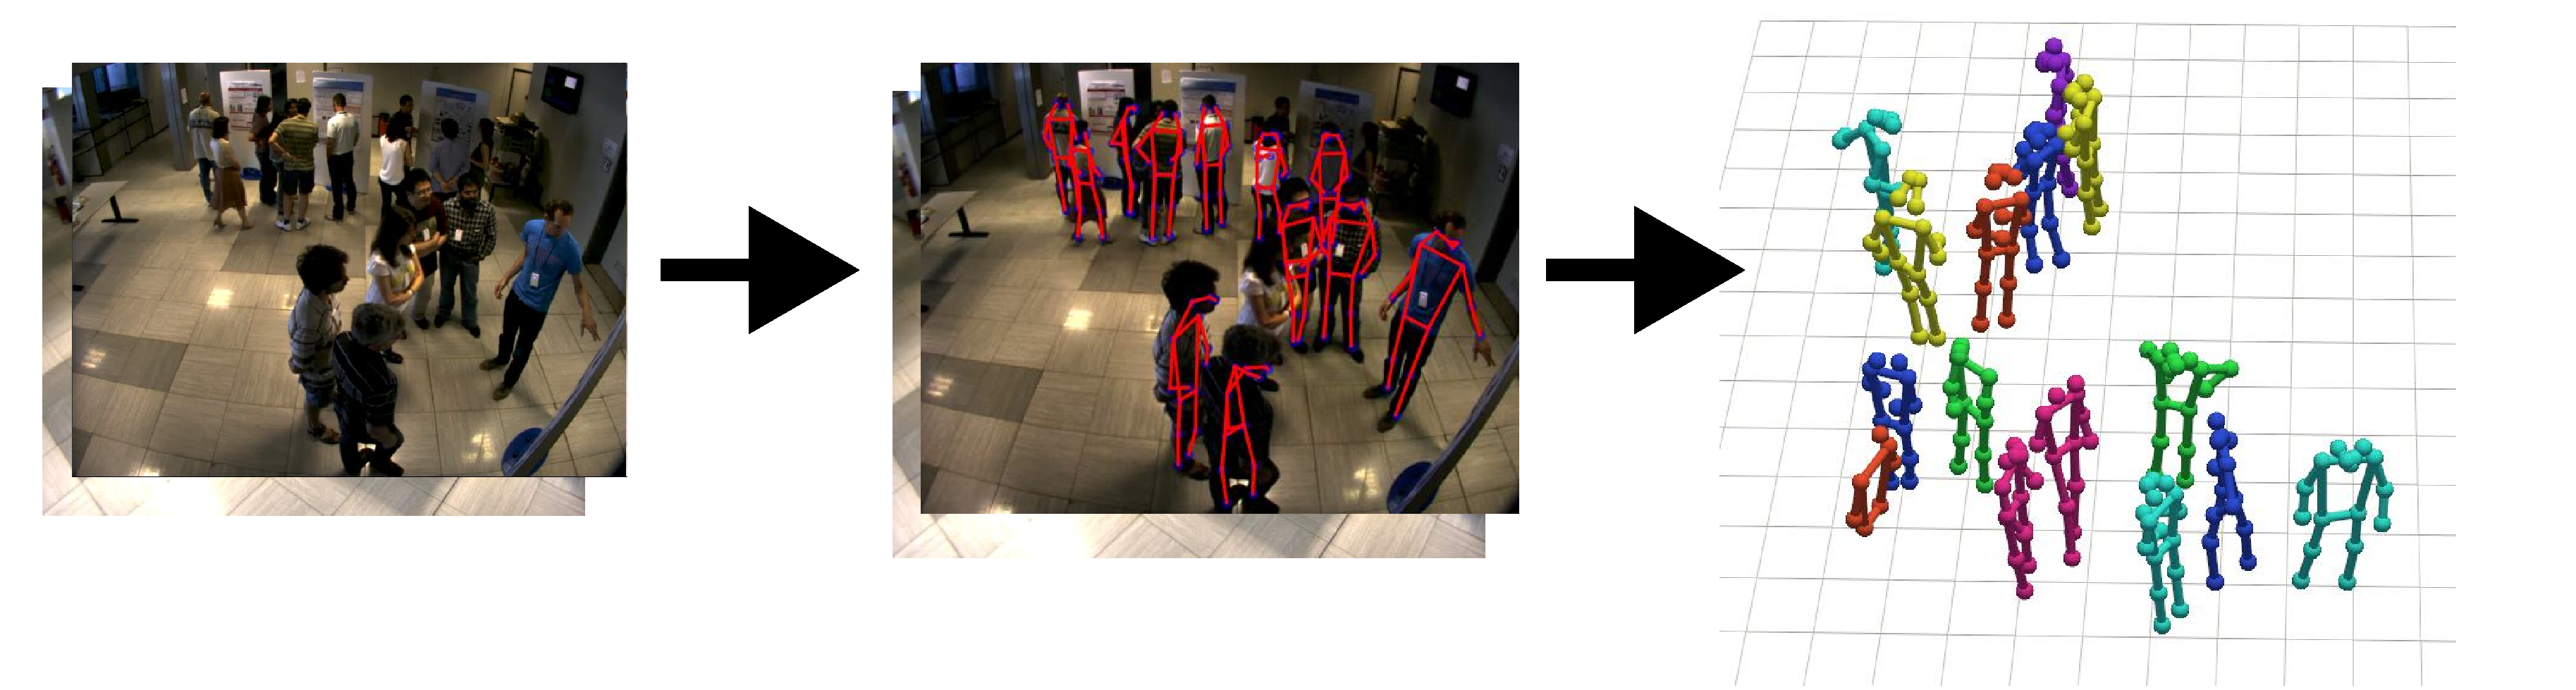
\includegraphics[width=0.9\linewidth]{figures/approach.pdf}
    \end{figure}
  \end{items}
\end{frame}

\begin{frame}
\frametitle{Task Formulation}
  \begin{items}
    \begin{oitem}{\litem}
      Given: \\
      \sitem {\footnotesize Multiple video sequences containing multiple people.} \\
      \sitem {\footnotesize Recorded synchronously from multiple camera views.} \\
      \sitem {\footnotesize Camera calibration parameters, including extrinsics, intrinsic and distortion.}
    \end{oitem}
    \begin{oitem}{\litem}
      Output: \\
      \sitem {\footnotesize 3D coordinates of skeletal joints for each subject.} \\
      \sitem {\footnotesize Temporally consistent movement of skeletal joints over time.}
    \end{oitem}
    \begin{center}
      \begin{tikzpicture}[
          node distance=10mm,>=Latex,
          base_node/.style={minimum height=5mm,align=center,text width=3cm},
          icon_node/.style={minimum size=7mm,align=center}
      ]
          \node (satellite) [icon_node] {\fontsize{40pt}{40pt}\selectfont\faVideo};
          \node [below=1mm of satellite, font=\scriptsize] {Calibrated Cameras};
          \node [base_node, right=of satellite, inner sep=-5mm, yshift=6, xshift=6] {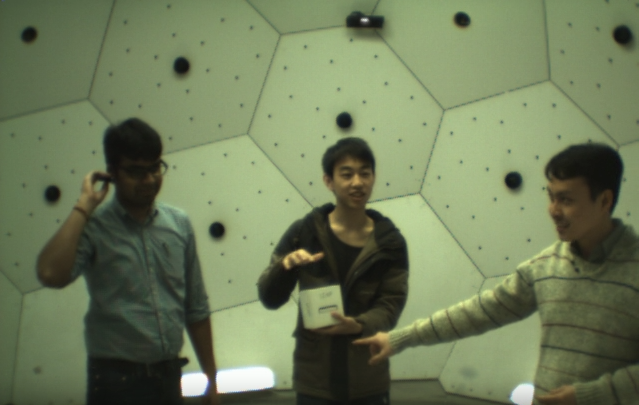
\includegraphics[width=15mm]{figures/examples/example1.png}};
          \node [base_node, right=of satellite, inner sep=-5mm, yshift=4, xshift=4] {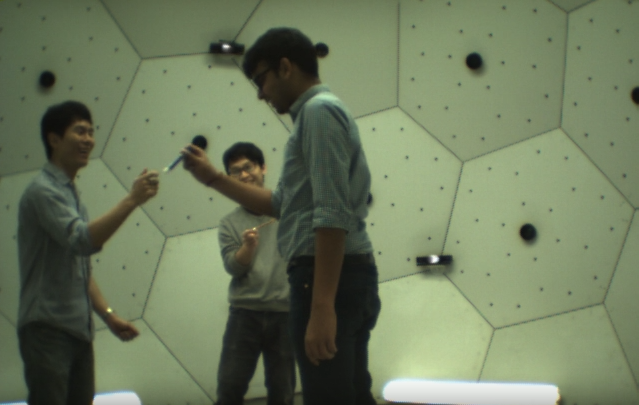
\includegraphics[width=15mm]{figures/examples/example2.png}};
          \node [base_node, right=of satellite, inner sep=-5mm, yshift=2, xshift=2] {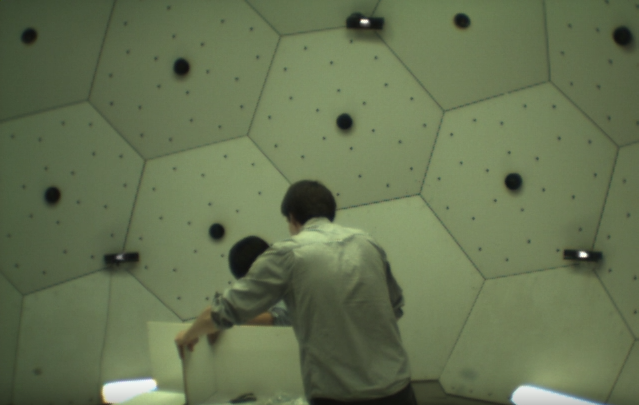
\includegraphics[width=15mm]{figures/examples/example3.png}};
          \node (image_data) [base_node, right=of satellite, inner sep=-5mm] {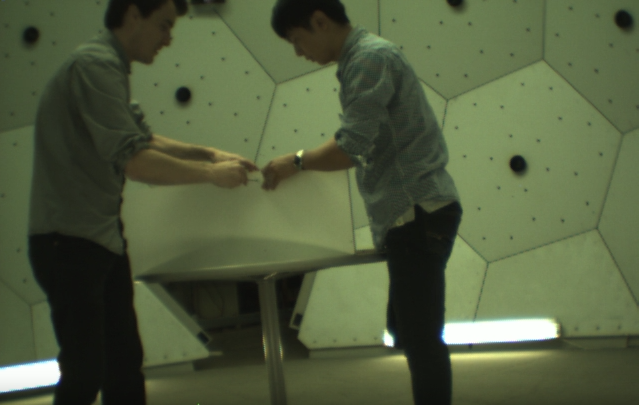
\includegraphics[width=15mm]{figures/examples/example4.png}};
          \node [below=6.25mm of image_data, font=\scriptsize] {Multi-View Video};
          \node (machine_learning) [icon_node, right=of image_data] {
            \fontsize{40pt}{40pt}\selectfont\faRobot
          };
          \node [below=1mm of machine_learning, font=\scriptsize] {CV System};
          \node (pred) [base_node, right=of machine_learning, inner sep=-5mm] {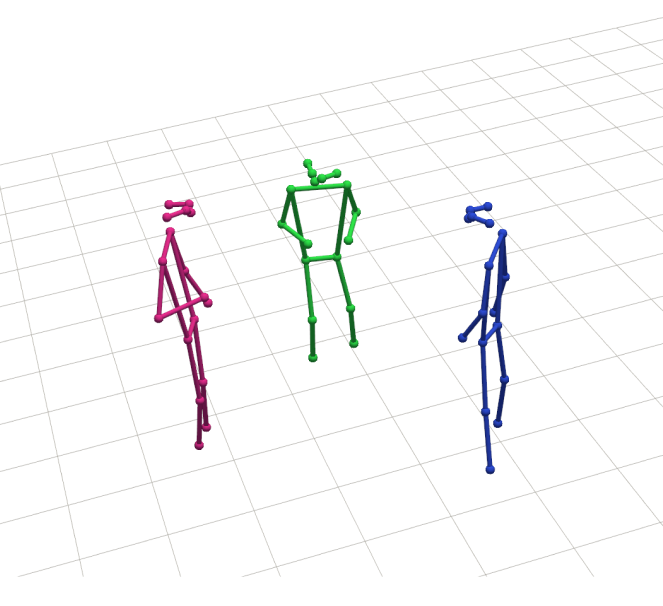
\includegraphics[width=15mm]{figures/example-out.png}};
          \node [below=6.25mm of pred, font=\scriptsize] {Predict 3D Skeletons};
          \draw[->, thick] (satellite) -- (image_data);
          \draw[->, thick] (image_data) -- (machine_learning);
          \draw[->, thick] (machine_learning) -- (pred);
      \end{tikzpicture}
    \end{center}
  \end{items}
\end{frame}

\begin{frame}
\frametitle{System Architecture -- Overview}
  \begin{items}
    \begin{oitem}{\litem}
      Summary: \\
      \sitem {\footnotesize Perform single-view single-frame 2D estimation using pretrained model.} \\
      \sitem {\footnotesize Cross-view and prediction-view matching of detections using Mahalanobis distance.} \\
      \sitem {\footnotesize Fusion of 2D observations into 3D skeletal trajectories using extended Kalman filter.}
    \end{oitem}
    \input{tikzfigures/architecture.tex}
  \end{items}
\end{frame}

\begin{frame}
\frametitle{System Architecture -- 2D Detections}
  \begin{items}
    \begin{oitem}{\litem}
      Summary: \\
      \sitem {\footnotesize Using YOLO26-pose family of models for the detector.} \\
      \sitem {\footnotesize Dynamically scale observation covariances based on YOLO keypoint confidence.} \\
      \sitem {\footnotesize Transform 2D pixel coordinates into normalized camera coordinates.}
    \end{oitem}
    \input{tikzfigures/detection.tex}
  \end{items}
\end{frame}

\begin{frame}
\frametitle{System Architecture -- Data Association}
  \begin{items}
    \begin{oitem}{\litem}
      Two-step process: \\
      \sitem {\footnotesize For each view, try to associate detections to predicted 3D state.} \\
      \sitem {\footnotesize For all unmatched detections, try to associate between different views.}
    \end{oitem}
    \begin{oitem}{\litem}
      For all cross-view matches: \\
      \sitem {\footnotesize Triangulate 3D keypoint locations using all matched views to initialize tracks.}
    \end{oitem}
    \vspace*{-6mm}
    \input{tikzfigures/association.tex}
  \end{items}
\end{frame}

\begin{frame}
\frametitle{System Architecture -- Extended Kalman Filtering}
  \begin{items}
    \begin{oitem}{\litem}
      Summary: \\
      \sitem {\footnotesize State representation contains 3D position and velocity for each keypoint.} \\
      \sitem {\footnotesize Prediction uses standard linear velocity model.} \\
      \sitem {\footnotesize All associated observations are concatenated and considered at once.} \\
      \sitem {\footnotesize Since the observation process is non-linear extended Kalman filtering is used.}
    \end{oitem}
    \input{tikzfigures/kalman.tex}
  \end{items}
\end{frame}

\begin{frame}
\frametitle{Skeletal Constraints}
  \begin{items}
    \begin{oitem}{\litem}
      Summary: \\
      \sitem {\footnotesize Assume limb lengths do not change and are left-right symmetrical.} \\
      \sitem {\footnotesize Adding length values to the state vector of the filter.} \\
      \sitem {\footnotesize No direct interaction with other state values and very low process noise.} \\
      \sitem {\footnotesize Pseudo-observation merged into each update step that observes constraint violation of 0.}
    \end{oitem}
    \begin{columns}[c]
      \begin{column}{0.85\textwidth}
        \begin{align*}
            \mathbf{x} &= \begin{bmatrix} \mathbf{p}_1^T, \; \dots, \; \mathbf{p}_{17}^T, \; \mathbf{v}_1^T, \; \dots, \; \mathbf{v}_{17}^T, \; l_1, \; \dots, \; l_{12} \end{bmatrix}^T
        \end{align*}
        \begin{align*}
            h_\mathrm{sc}(\mathbf{x}) &= \begin{bmatrix} \rho_1(\mathbf{x}) & \rho_2(\mathbf{x}) & \dots & \rho_{20}(\mathbf{p}) \end{bmatrix}^T
        \end{align*}
        \begin{align*}
            \rho_j(\mathbf{x}) &= \|\mathbf{p}_{a_j} - \mathbf{p}_{b_j}\|_2 - l_{i_j} \quad \quad \quad \mathbf{z}_\mathrm{sc} = 0
        \end{align*}
      \end{column}
      \begin{column}{0.15\textwidth}
        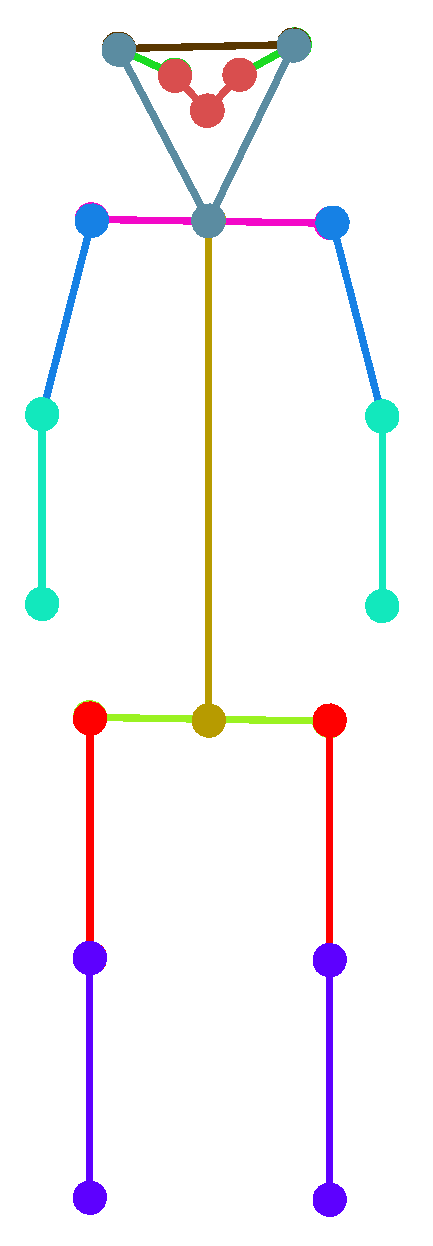
\includegraphics[width=0.7\linewidth]{figures/skeleton.pdf}
      \end{column}
    \end{columns}
  \end{items}
\end{frame}

\begin{frame}
\frametitle{Learning Parameters from Data}
  \begin{items}
    % TODO
    \begin{oitem}{\litem}
      Summary: \\
      \sitem {\footnotesize Learning the complete pipeline end-to-end unfeasible.} \\
      \sitem {\footnotesize Split the learning into three independent parts that are learned separately.} \\
      \sitem {\footnotesize Training is done using the CMU Panoptic dataset excluding sequences used for testing.} \\
      \sitem {\footnotesize Se.}
    \end{oitem}
    \begin{figure}
      \centering
      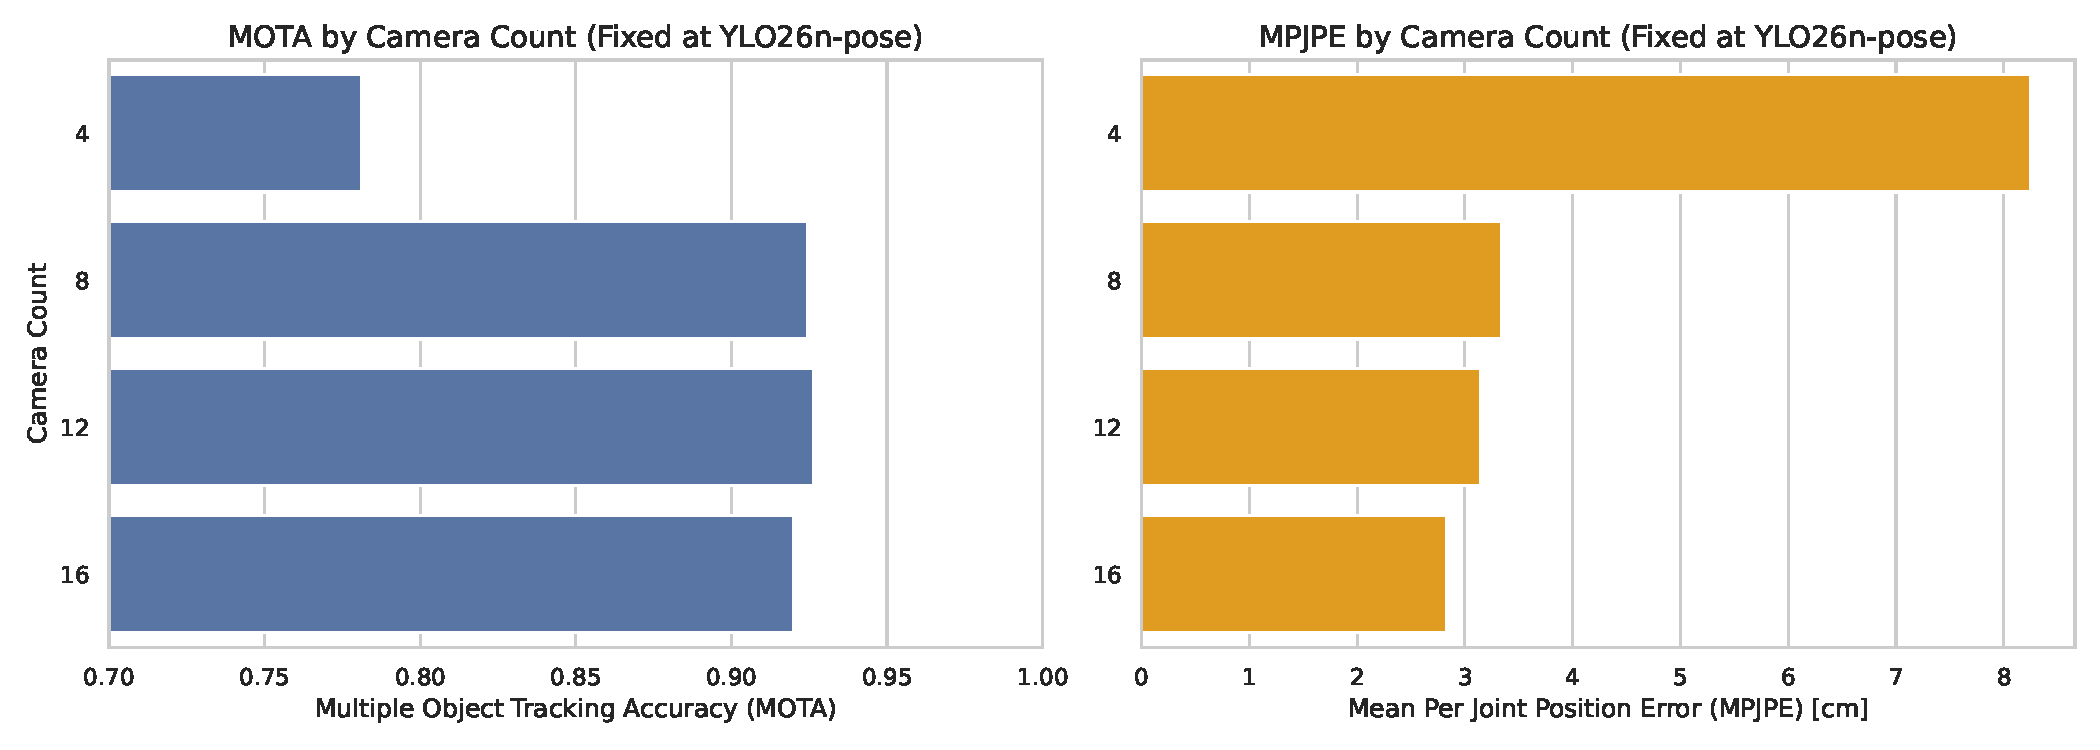
\includegraphics[width=\linewidth]{figures/camera_count_comparison.pdf}
    \end{figure}
  \end{items}
\end{frame}

\begin{frame}
\frametitle{Learning Parameters from Data -- Custom YOLO Head}
  \begin{items}
    % TODO
    \begin{oitem}{\litem}
      Summary: \\
      \sitem {\footnotesize Ipsum laborum incidunt consequatur nobis.} \\
      \sitem {\footnotesize Consequuntur repudiandae non odio sunt consequatur alias.} \\
      \sitem {\footnotesize Magni esse et non quas eveniet molestias quidem aut.} \\
      \sitem {\footnotesize Id ut nihil aut et numquam.}
    \end{oitem}
    \begin{figure}
      \centering
      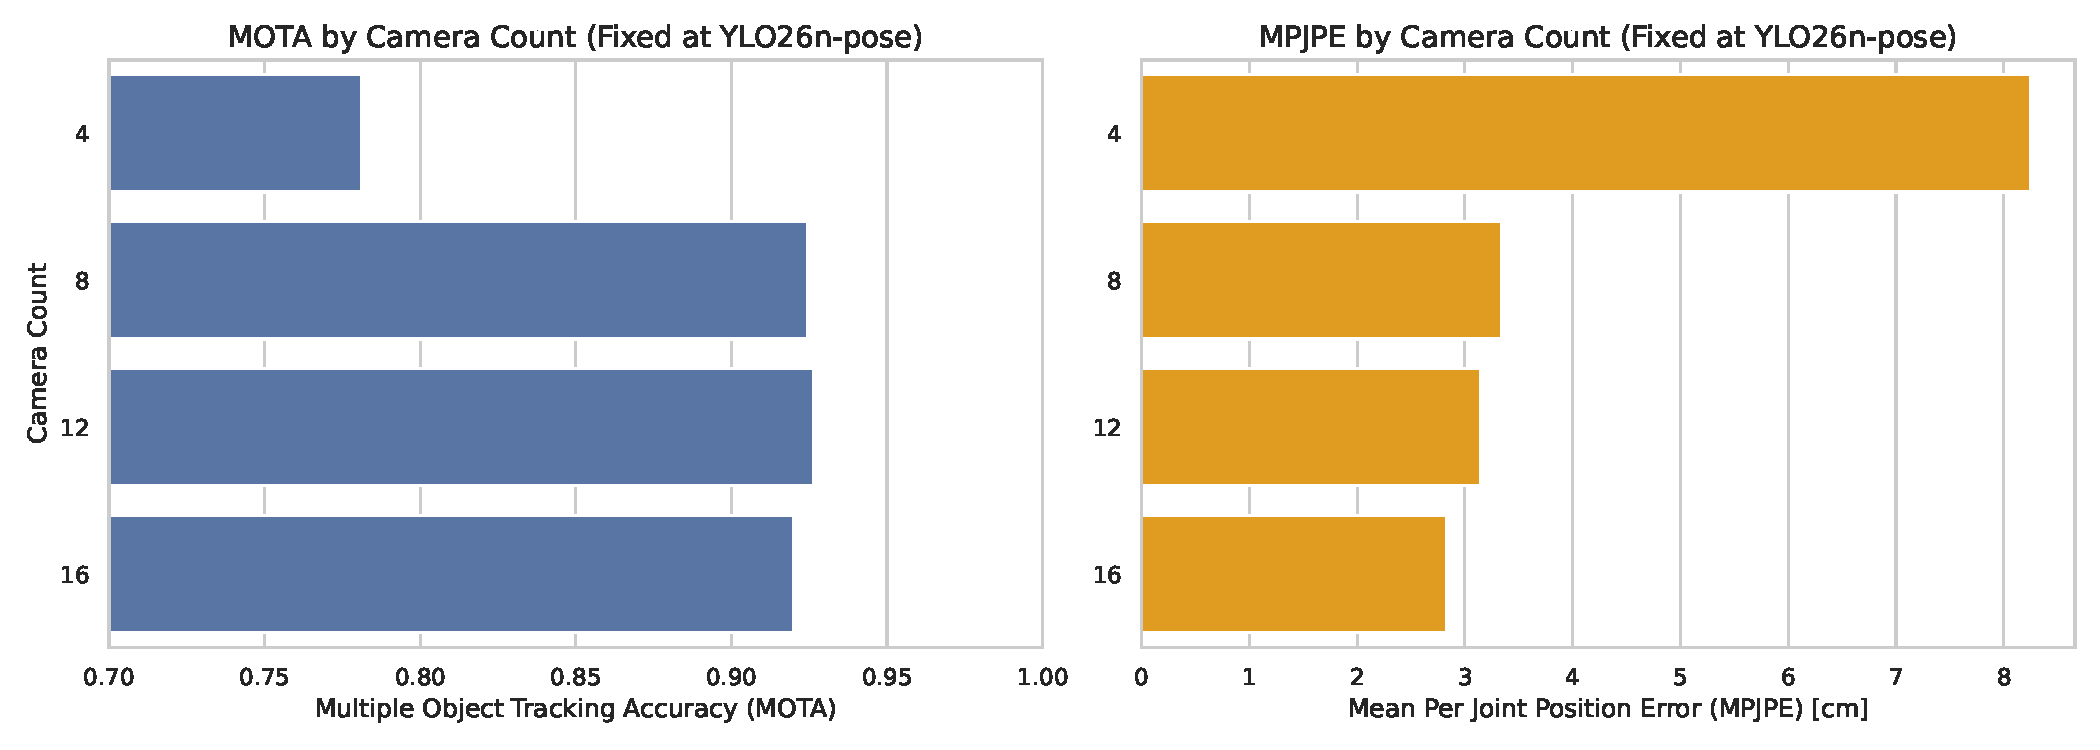
\includegraphics[width=\linewidth]{figures/camera_count_comparison.pdf}
    \end{figure}
  \end{items}
\end{frame}

\begin{frame}
\frametitle{Learning Parameters from Data -- Kalman Filter}
  \begin{items}
    % TODO
    \begin{oitem}{\litem}
      Summary: \\
      \sitem {\footnotesize Ipsum laborum incidunt consequatur nobis.} \\
      \sitem {\footnotesize Consequuntur repudiandae non odio sunt consequatur alias.} \\
      \sitem {\footnotesize Magni esse et non quas eveniet molestias quidem aut.} \\
      \sitem {\footnotesize Id ut nihil aut et numquam.}
    \end{oitem}
    \begin{figure}
      \centering
      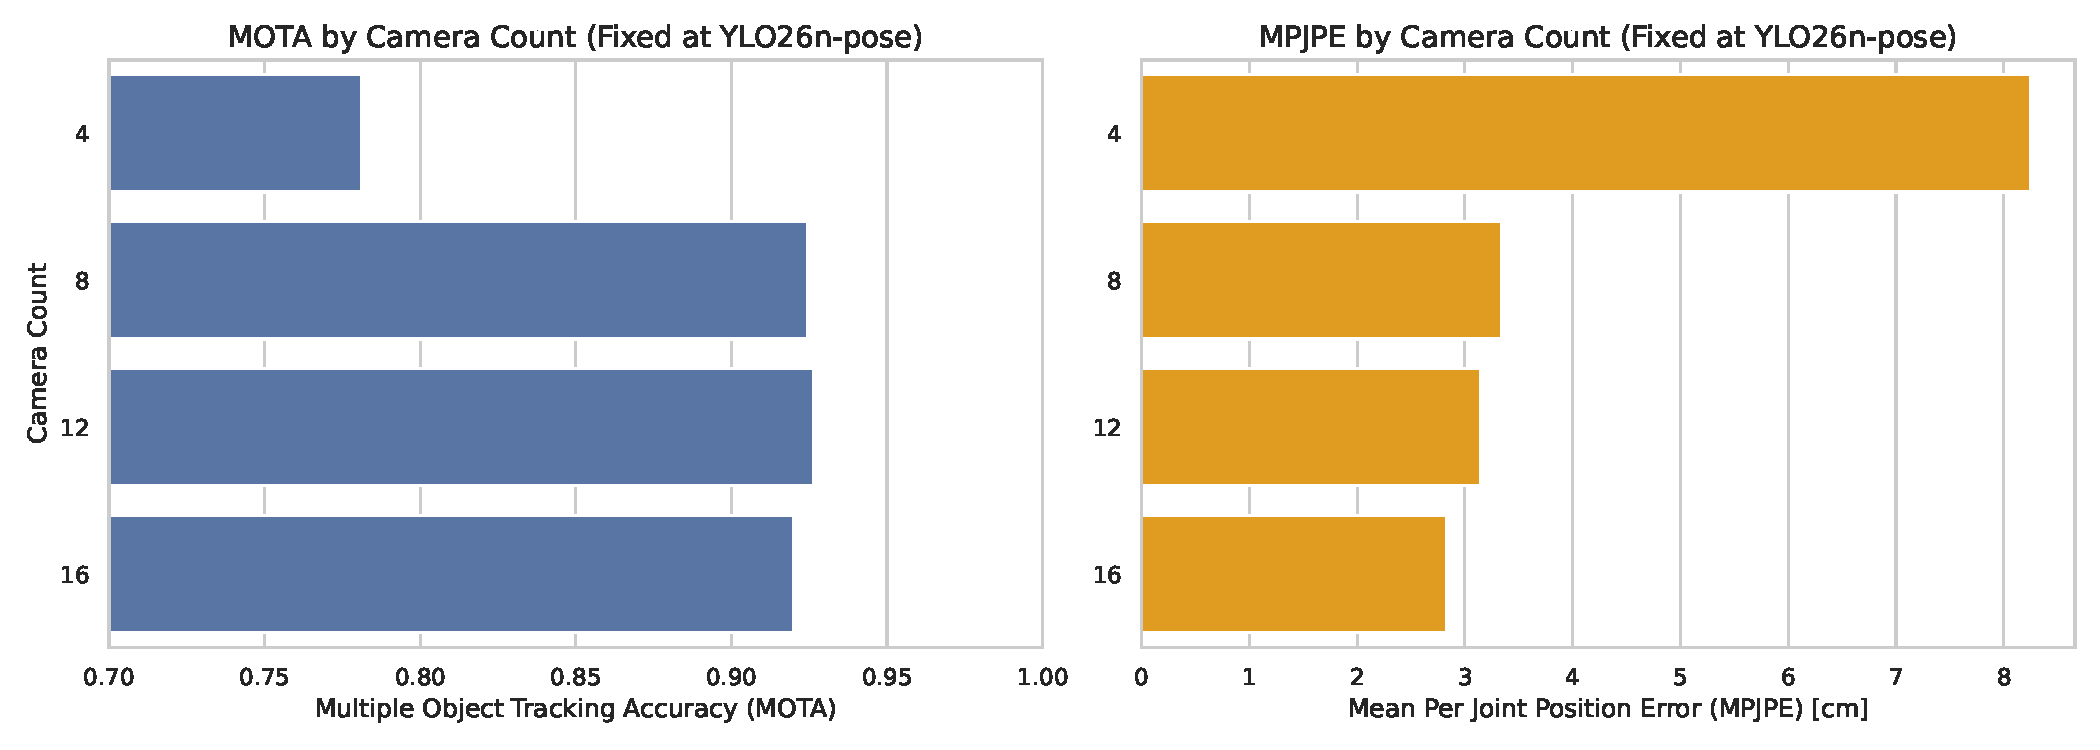
\includegraphics[width=\linewidth]{figures/camera_count_comparison.pdf}
    \end{figure}
  \end{items}
\end{frame}

\begin{frame}
\frametitle{Dataset Overview -- CMU Panoptic Dataset}
  \begin{items}
    \begin{oitem}{\litem}
      Source: \\
      \sitem {\footnotesize Video captured in a specialized 5.49m diameter dome-shaped room.} \\
      \sitem {\footnotesize Equipped with hundreds of inward facing cameras attached to the outside panels.}
    \end{oitem}
    \begin{oitem}{\litem}
      Format and Data Characteristics: \\
      \sitem {\footnotesize 84 video sequences totaling approximately 11.5 hours of video.} \\
      \sitem {\footnotesize VGA cameras recording at a 640×480 resolution
at 25 fps.} \\
      \sitem {\footnotesize Includes ground truth 3D skeletons and
tracks n COCO19 format.}
    \end{oitem}
    \begin{figure}
      \centering
      \begin{subfigure}[b]{0.59\textwidth}
        \begin{subfigure}[t]{\linewidth}
          \begin{subfigure}[t]{0.30\linewidth}
            \centering
            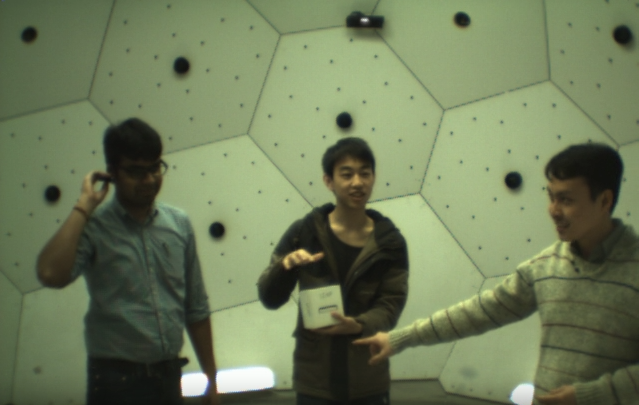
\includegraphics[width=\linewidth]{figures/examples/example1.png}
          \end{subfigure}
          \begin{subfigure}[t]{0.30\linewidth}
            \centering
            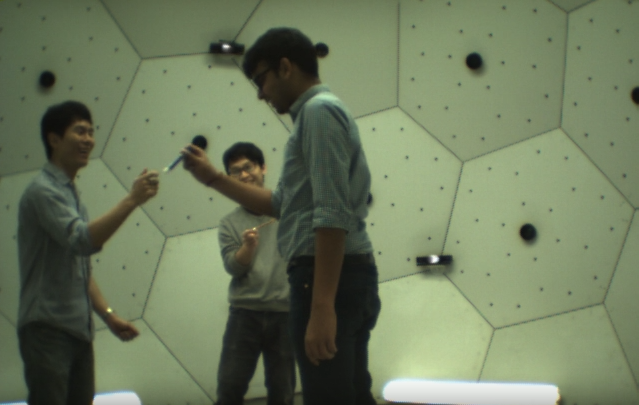
\includegraphics[width=\linewidth]{figures/examples/example2.png}
          \end{subfigure}
          \begin{subfigure}[t]{0.30\linewidth}
            \centering
            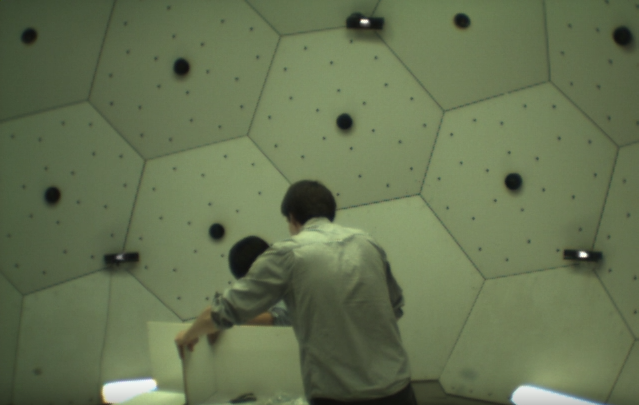
\includegraphics[width=\linewidth]{figures/examples/example3.png}
          \end{subfigure}
        \end{subfigure}
        \begin{subfigure}[t]{\linewidth}
          \begin{subfigure}[t]{0.30\linewidth}
            \centering
            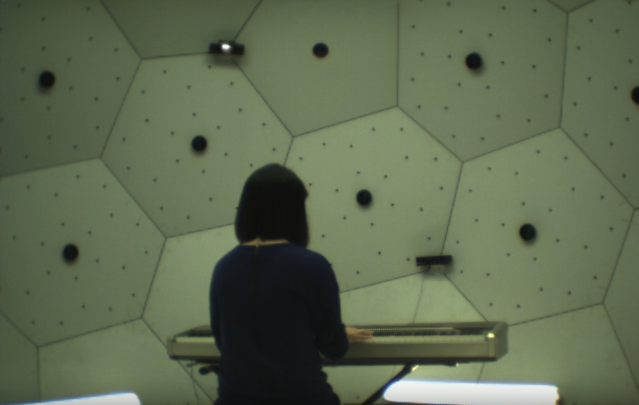
\includegraphics[width=\linewidth]{figures/examples/example6.png}
          \end{subfigure}
          \begin{subfigure}[t]{0.30\linewidth}
            \centering
            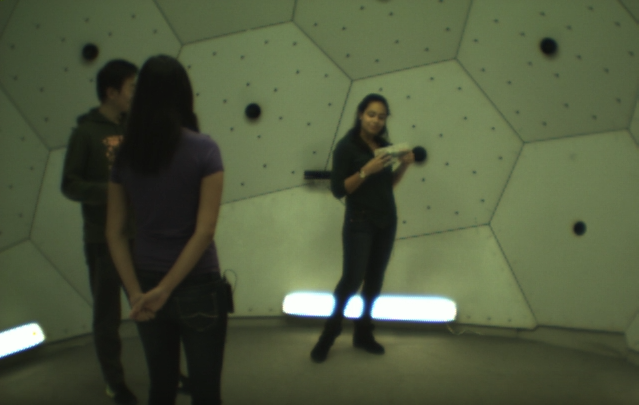
\includegraphics[width=\linewidth]{figures/examples/example7.png}
          \end{subfigure}
          \begin{subfigure}[t]{0.30\linewidth}
            \centering
            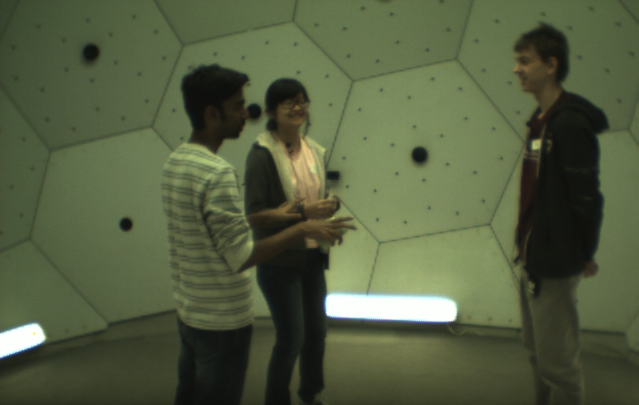
\includegraphics[width=\linewidth]{figures/examples/example8.png}
          \end{subfigure}
        \end{subfigure}
      \end{subfigure}
      \begin{subfigure}[b]{0.36\textwidth}
        \centering
        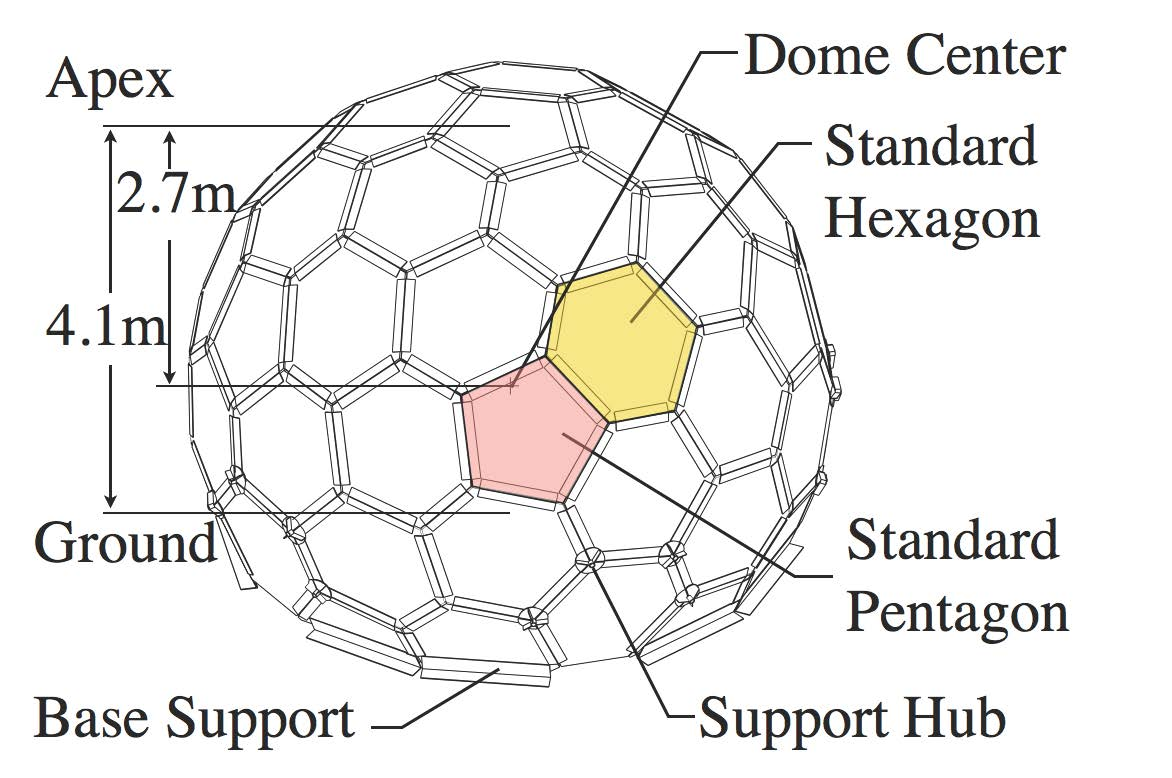
\includegraphics[width=\linewidth]{figures/cmu-panoptic.png}
      \end{subfigure}
    \end{figure}
  \end{items}
\end{frame}

\begin{frame}
\frametitle{Experimental Setup}
  \begin{items}
    \begin{oitem}{\litem}
      Setup: \\
      \sitem {\footnotesize Run evaluation on a subset of 8 sequences from the dataset.} \\
      \sitem {\footnotesize Compare generated pose tracks against ground truth annotations.} \\
      \sitem {\footnotesize Evaluate using variating number of camera views and differently sized YOLO models.} \\
      \sitem {\footnotesize Also record timing statistics for evaluation of algorithm efficiency.}
    \end{oitem}
    \begin{oitem}{\litem}
      Evaluation Metrics: \\
      \sitem {\footnotesize Mean Per-Joint Position Error (MPJPE).} \\
      \sitem {\footnotesize Multi-Object Tracking Accuracy (MOTA).} \\
      \sitem {\footnotesize Also collected Precision and Recall.}
    \end{oitem}
  \end{items}
\end{frame}

\begin{frame}
\frametitle{Quantitative Results -- Runtime Efficiency}
  \begin{items}
    \begin{oitem}{\litem}
      Main Finding: \\
      \sitem {\footnotesize Detection is the largest part of the execution time per frame.} \\
      \sitem {\footnotesize Execution time of detection scales linearly with number of cameras.} \\
      \sitem {\footnotesize Matching and filtering also scale with camera count but slight less quickly.}
    \end{oitem}
    \begin{widepage}
      \begin{figure}
        \centering
        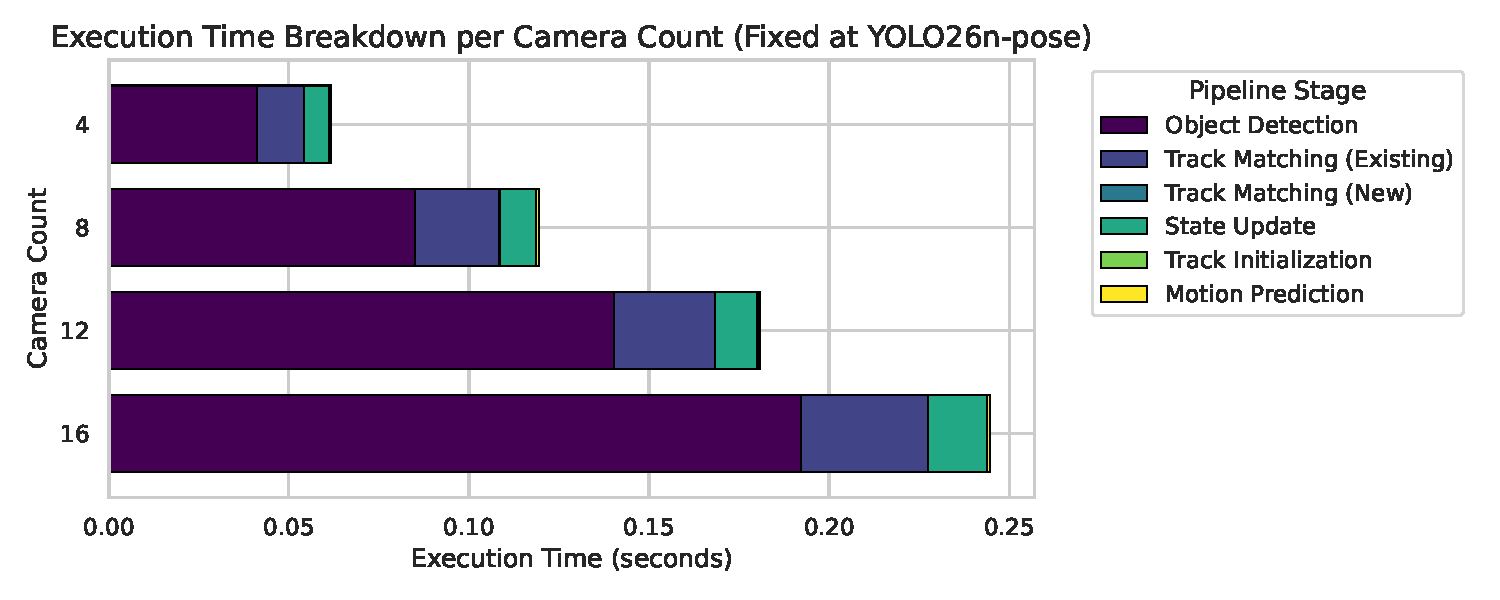
\includegraphics[width=\linewidth]{figures/execution_time_breakdown_cams.pdf}
      \end{figure}
    \end{widepage}
  \end{items}
\end{frame}

\begin{frame}
\frametitle{Quantitative Results -- Performance vs. Model Size}
  \begin{items}
    \begin{oitem}{\litem}
      Main Finding: \\
      \sitem {\footnotesize Larger models improve both MOTA and MPJPE metrics.} \\
      \sitem {\footnotesize Especially large version gives good results.} \\
      \sitem {\footnotesize Small and medium version are not significantly better than nano version.}
    \end{oitem}
    \begin{widepage}
      \begin{figure}
        \centering
        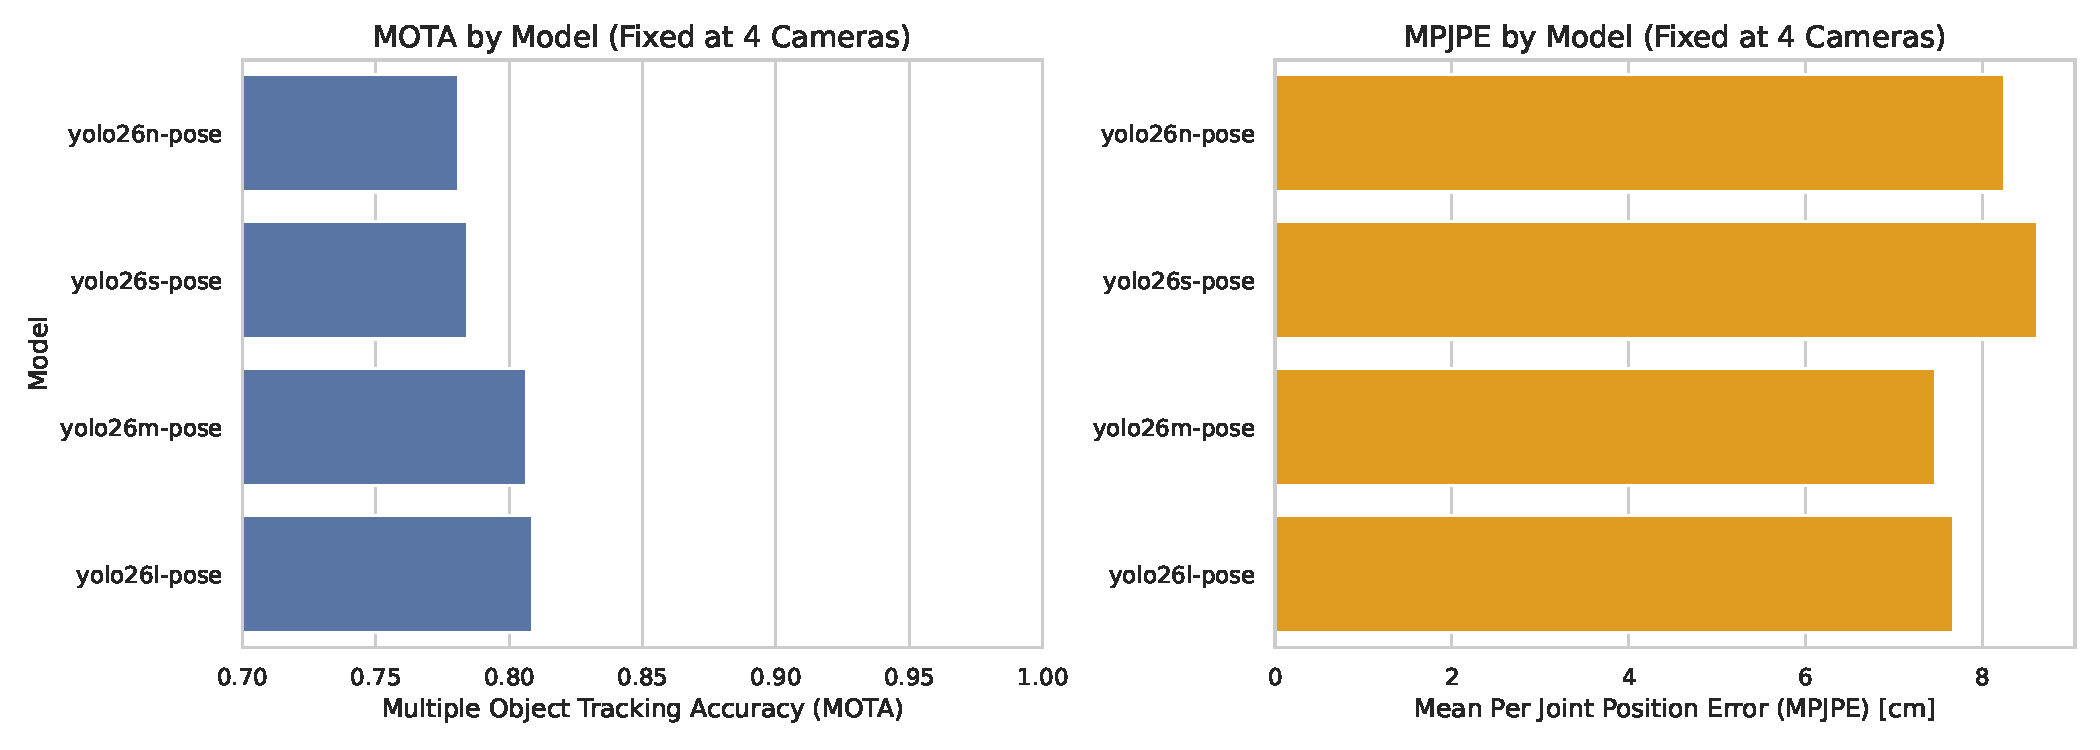
\includegraphics[width=\linewidth]{figures/model_comparison_4_cams.pdf}
      \end{figure}
    \end{widepage}
  \end{items}
\end{frame}

\begin{frame}
\frametitle{Quantitative Results -- Performance vs. Camera Count}
  \begin{items}
    \begin{oitem}{\litem}
      Main Finding: \\
      \sitem {\footnotesize Adding more cameras significantly improves MPJPE.} \\
      \sitem {\footnotesize Additional views slightly reduce MOTA due to more false positives.} \\
      \sitem {\footnotesize More camera views is more effective than larger model capacity for MPJPE.}
    \end{oitem}
    \begin{widepage}
      \begin{figure}
        \centering
        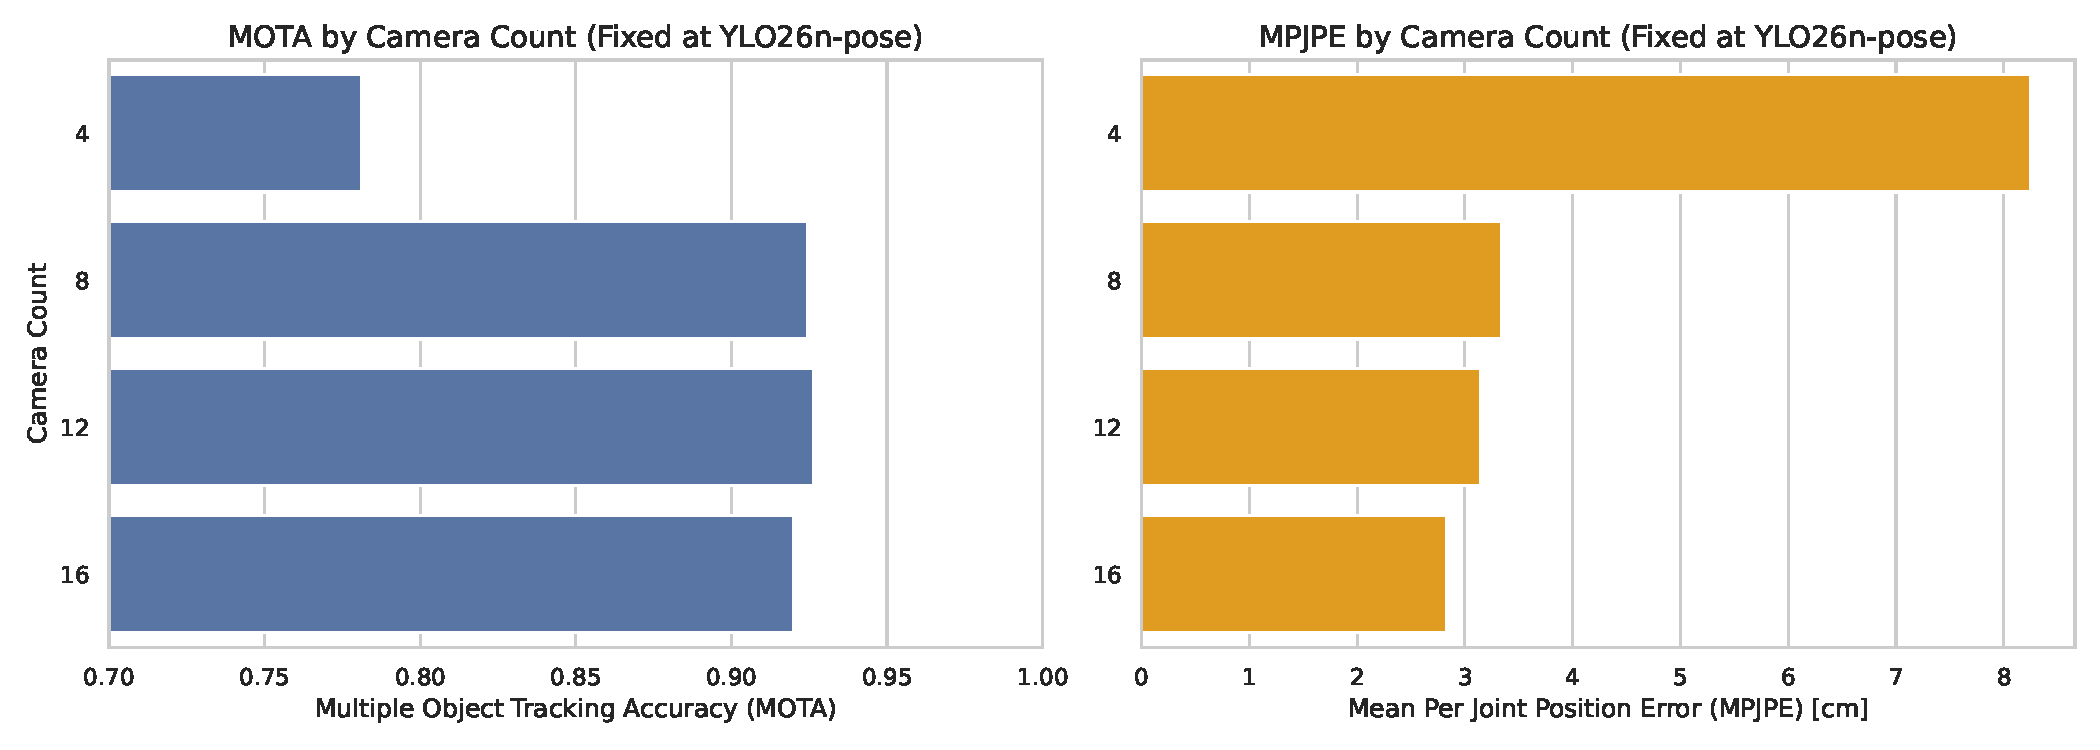
\includegraphics[width=\linewidth]{figures/camera_count_comparison.pdf}
      \end{figure}
    \end{widepage}
  \end{items}
\end{frame}

\begin{frame}
\frametitle{Quantitative Results -- Skeletal Constraints and Learning}
  \begin{items}
    \begin{oitem}{\litem}
      Main Finding: \\
      \sitem {\footnotesize Ipsum laborum incidunt consequatur nobis.} \\
      \sitem {\footnotesize Consequuntur repudiandae non odio sunt consequatur alias.} \\
      \sitem {\footnotesize Id ut nihil aut et numquam.}
    \end{oitem}
    \begin{widepage}
      \begin{figure}
        \centering
        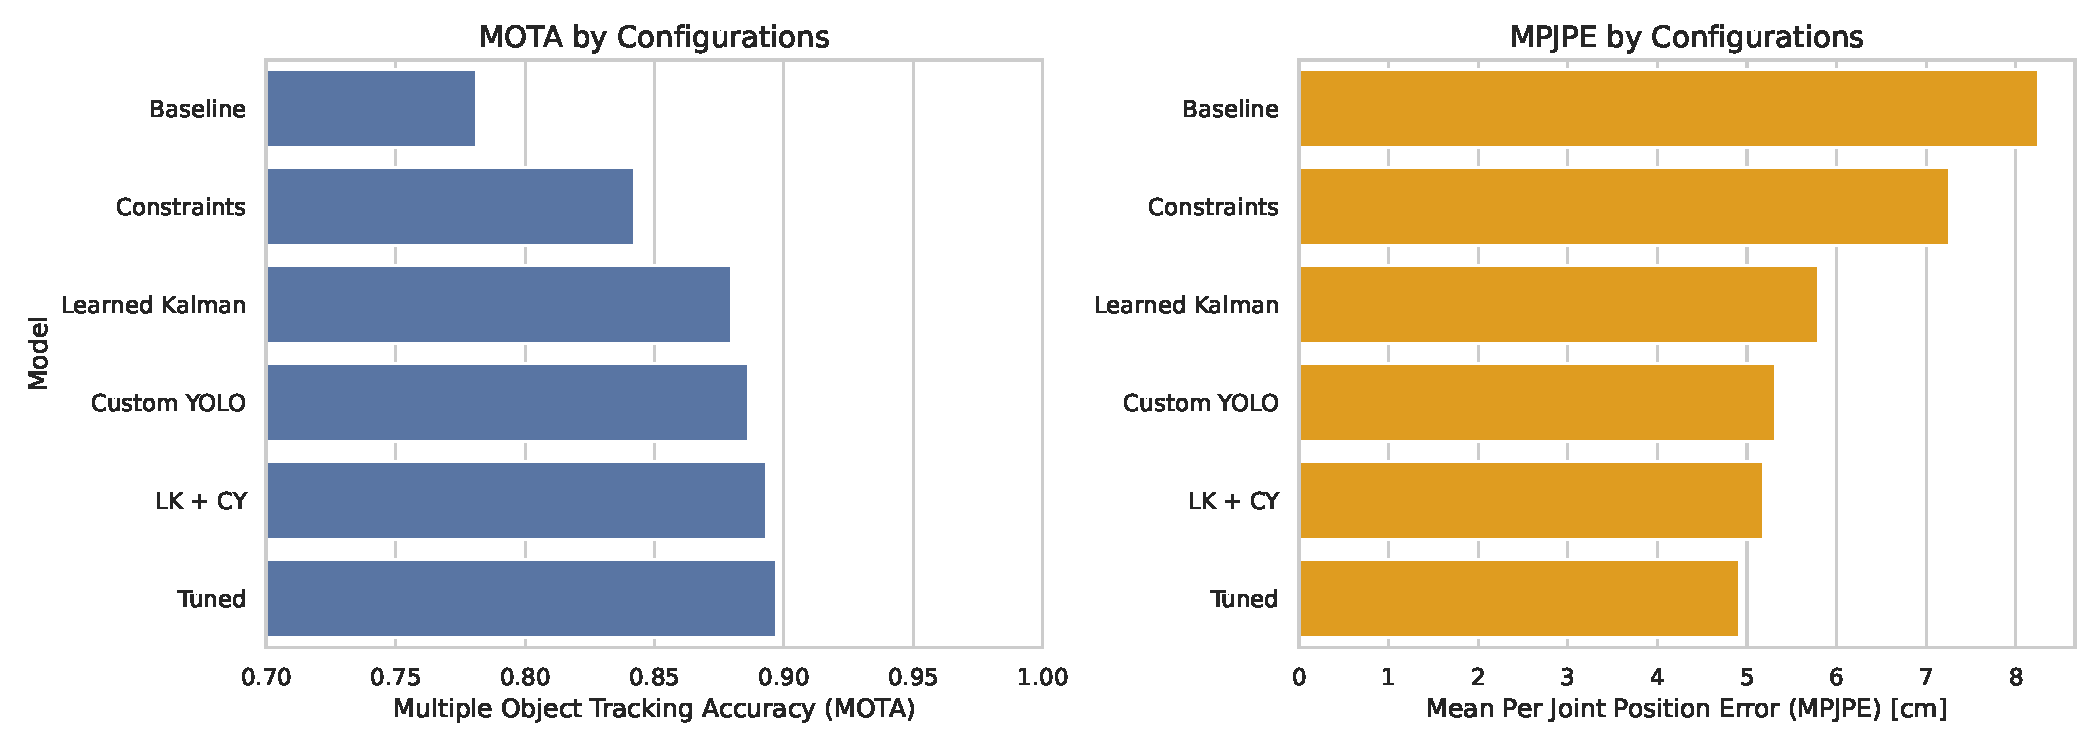
\includegraphics[width=\linewidth]{figures/improvements_comparison_4_cams.pdf}
      \end{figure}
    \end{widepage}
  \end{items}
\end{frame}

\begin{frame}
\frametitle{Qualitative Results}
  \begin{items}
    \begin{oitem}{\litem}
      Common failure modes: \\
      \sitem {\footnotesize Partially occluded persons keypoints drifting.} \\
      \sitem {\footnotesize Inactive track seen by only one camera can not cause track creation.} \\
      \sitem {\footnotesize Active track seen by only one camera can cause drift.} \\
      \sitem {\footnotesize Detection of person while exiting when ground truth is missing.}
    \end{oitem}
    \begin{figure}
      \centering
      \hfill
      \begin{subfigure}[t]{0.19\linewidth}
        \centering
        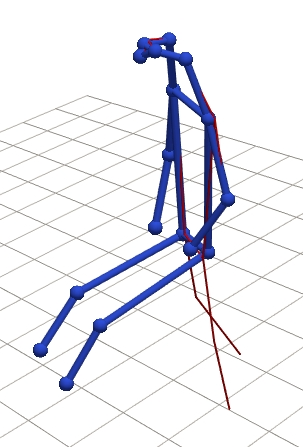
\includegraphics[width=\linewidth]{figures/qualitative1.png}
      \end{subfigure}
      \hfill
      \begin{subfigure}[t]{0.19\linewidth}
        \centering
        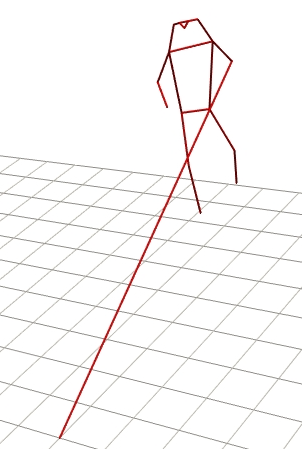
\includegraphics[width=\linewidth]{figures/qualitative2.png}
      \end{subfigure}
      \hfill
      \begin{subfigure}[t]{0.19\linewidth}
        \centering
        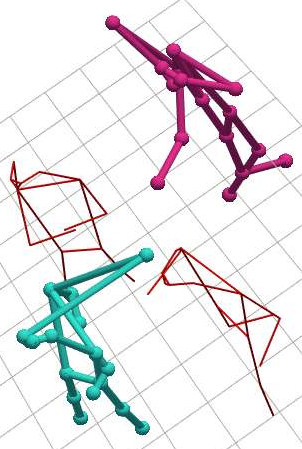
\includegraphics[width=\linewidth]{figures/qualitative3.png}
      \end{subfigure}
      \hfill
      \begin{subfigure}[t]{0.19\linewidth}
        \centering
        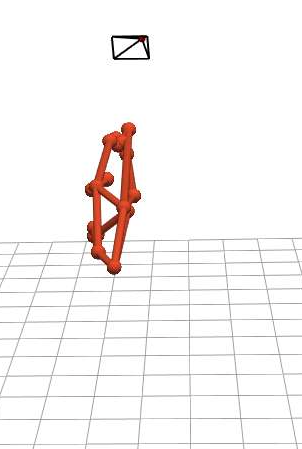
\includegraphics[width=\linewidth]{figures/qualitative4.png}
      \end{subfigure}
      \hfill
    \end{figure}
  \end{items}
\end{frame}

\begin{frame}
\frametitle{Conclusion}
  \begin{items}
    \begin{oitem}{\litem}
      Summary: \\
      \sitem {\footnotesize Implemented an EKF framework that merges multi-view observations.} \\
      \sitem {\footnotesize Incorporated skeletal length consistency constraints.} \\
      \sitem {\footnotesize Implemented simple learning of parameters from data.} \\
      \sitem {\footnotesize Analyzed performance across different system configuration.}
    \end{oitem}
    \begin{oitem}{\litem}
      Limitations: \\
      \sitem {\footnotesize Still struggles significantly with occlusions.} \\
      \sitem {\footnotesize Running 2D pose estimation remains a performance bottleneck.}
    \end{oitem}
    \begin{oitem}{\litem}
      Possible Future Improvements: \\
      \sitem {\footnotesize Add more constraints that force other known properties, such as joint angles.}\\
      \sitem {\footnotesize Find more stable learning methods for the Kalman filter parameters.} \\
      \sitem {\footnotesize Use of a particle filter with occlusion aware likelihood.}
    \end{oitem}
  \end{items}
\end{frame}


{
\setbeamercolor{background canvas}{bg=black}
\begin{frame}[plain]{}
\end{frame}
}

\end{document}
